\emph{Tekniskt sett kan radioamatörerna världen över, med hjälp av
  sina radiostationer, tämligen lätt skapa kontakt med
  varandra. Därvid krävs att reglerna i de länder som berörs vid
  kontakten respekteras.}

\emph{En hel serie både internationella och nationella regler styr
  radiokommunikationerna i en nation. Varje radioamatör skall känna
  till och följa dessa regler så långt de har anslutning till
  amatörradio. Vissa länder - t.ex. CEPT-länderna - har i någon
  utsträckning harmoniserat sina bestämmelser inbördes.  Nationella
  avvikelser förekommer likväl och reglerna i det land, som man gör
  radiosändningar ifrån, skall alltid följas.}

\section{ITU Radioreglemente (RR)}

Amatör- och Amatörsatellittjänsterna är radiokommunikationstjänster
med syfte att tillhandahålla nödvändig kommunikation i händelse av
naturkatastrofer, träna operatörer och tekniker i radio- och
telekommunikationsteknik till ingen kostnad för stat och samhälle,
bidra till att tidsenlig radiokommunikation främjas och att förbättra
internationell förståelse och välvilja.

\subsection{Artikel 1 (RR) Termer och definitioner}
\textbf{
HAREC b.\ref{HAREC.c.1.1}\label{myHAREC.c.1.1},
 b.\ref{HAREC.c.1.2}\label{myHAREC.c.1.2}
}

S1.56 (RR) Amatörtjänst \\
En radiokommunikationstjänst avsedd för självutbildning, inbördes
kommunikation och tekniska undersökningar bedrivet av amatörer, det
vill säga av behörigen godkända personer intresserade av radioteknik,
endast av personligt intresse och utan ekonomiskt syfte.

S1.57 (RR) Amatörsatellittjänst \\
En radiokommunikationstjänst som använder rymdstationer på
jordsatelliter för samma ändamål som för Amatörradiotjänsten.  81.96
(RR) Amatörradiostation Radiostation inom amatörradiotjänst

S1.96 (RR) Amatörradiostation \\
Radiostation inom amatörradiotjänst.

\subsection{Artikel S25 (RR) (f.d. Artikel 32)}
\textbf{
HAREC b.\ref{HAREC.c.1.3}\label{myHAREC.c.1.3},
 b.\ref{HAREC.c.1.4}\label{myHAREC.c.1.4}
}

\subsubsection{Sektion I. Amatörtjänst}
S25.1 \# 1. Radiokommunikation mellan amatörstationer i olika länder
skall vara förbjuden, om administrationen i en av de berörda
nationerna har meddelat att den är emot sådan radiokommunikation.

S25.2 \# 2. (1) När sändningar mellan amatörstationer i olika !änder är
tillåtna, skall det ske på klart språk och begränsas till meddelanden
av teknisk natur i samband med prov och till personliga kommentarer,
som på grund av sin oviktighet inte är skäl nog för att ta den
allmänna telekommunikationstjänsten i anspråk.

S25.3 (2) Det är absolut förbjudet att använda amatörradiostationer
för internationell radiokommunikation för tredje parts räkning.

S25.4 (3) De föregående bestämmelserna får ändras genom särskilda
överenskommelser mellan administrationerna i berörda länder.

S25.5 \#3 (1) Varje person som söker en licens för att använda
apparaterna i en amatörradiostation skall bevisa sin förmåga att för
hand sända rätt och med hörseln rätt ta emot texter i form av
morsesignaler. Berörda administrationer får emellertid bortse från
detta krav för stationer som endast används på frekvenser över 30 MHz.

S25.6 (2) Administrationerna skall vidta sådana åtgärder som de finner
nödvändiga för att kontrollera de handhavandemässiga och tekniska
kvalifikationerna hos varje person som önskar använda apparaterna i en
amatörradiostation.

S25.7 \#4 Den högsta effekten från en amatörstation skall fastställas
av berörda administrationer, med hänsyn till operatörernas tekniska
kvalifikationer och under vilka förhållanden dessa stationer skall
användas.

S25.8 \#5 (1) Alla allmänna regler i överenskommelsen och de i denna
artikel skall tillämpas på amatörradiostationer. Särskilt den utsända
frekvensen skall vara så stabil och så fri från sidafrekvenser som den
tekniska utvecklingen för sådana stationer medger.

S25.9 (2) Under loppet av sändningarna skall amatörstationer sända
sina anropssignaler med korta mellanrum.

\subsection{Sektion II. Amatörsatellittjänst}

S25.10 \#6 Bestämmelserna i Sektion 1 i denna artikel skall gälla i all
tillämplig omfattning även för amatörsatellittjänst.

S25.10 \#7 Rymdstationer i amatörsatellittjänst, som arbetar i band som
delas med andra tjänster, skall förses med lämplig utrustning för att
kontrollera utstrålningen om skadlig störning rapporteras, allt i
överensstämmelse med den procedur som föreskrivs i Artikel S15
*.Administrationer som godkänner sådana rymdstationer skall informera
RRB (Radio Registrations Board) och skall tillse att tillfredställande
jordkontrollstationer upprättas före uppskjutningen för att
säkerställa att varje rapporterad skadlig störning skall kunna
avbrytas omedelbart av den bemyndigande administrationen. Se S22.1 **.

* S15 behandlar "lnterference"

** 822 behandlar "Space Services"

\subsection{Artikel 8 (RR 8-1) Frekvenstilldelning}

\subsubsection{Inledning}

391 § 1. I Unionens alla dokument där termerna \emph{allocation},
\emph{allotment} och \emph{assignment} används skall de ha den
betydelse som ges i nummer 17 till 19, varvid termerna på de tre
arbetsspråken skall vara som följer (franska, engelska och spanska):

Frekvensfördelning till:
\begin{tabular}{lll}
  Tjänster & Allocation & (tilldelning) \\
  Områden & Allotment & (fördelning) \\
  Stationer & Assignment & (anvisning) .... etc. \\
\end{tabular}
(För enkelhetens skull återges här endast
betydelserna på engelska språket).

\subsubsection{Sektion I. Regioner och områden}
\textbf{
HAREC b.\ref{HAREC.c.1.5}\label{myHAREC.c.1.5}
}

392 § 2. Förtilldelning av frekvenserhar världen delats in i tre
Regioner så som visas på följande karta och som beskrivs i 393 till
399 .... etc.

\emph{ Det innebär att tilldelning, fördelning och anvisning av
  frekvenser mycket väl kan skilja mellan ITU-regionerna. Skillnaderna
  förklaras t.ex. av regionalt olika behovsstruktur, befolkning etc.}

\emph{Det förekommer också likheter. På nedanstående karta har
  markerats en tropisk zon, vilket förklaras av den annorlunda
  vågutbredningen där. T.ex. behöver särskild hänsyn tas vid
  frekvenstilldelning (allokering) till rundradiotjänsten i zonen.}

\begin{figure}
  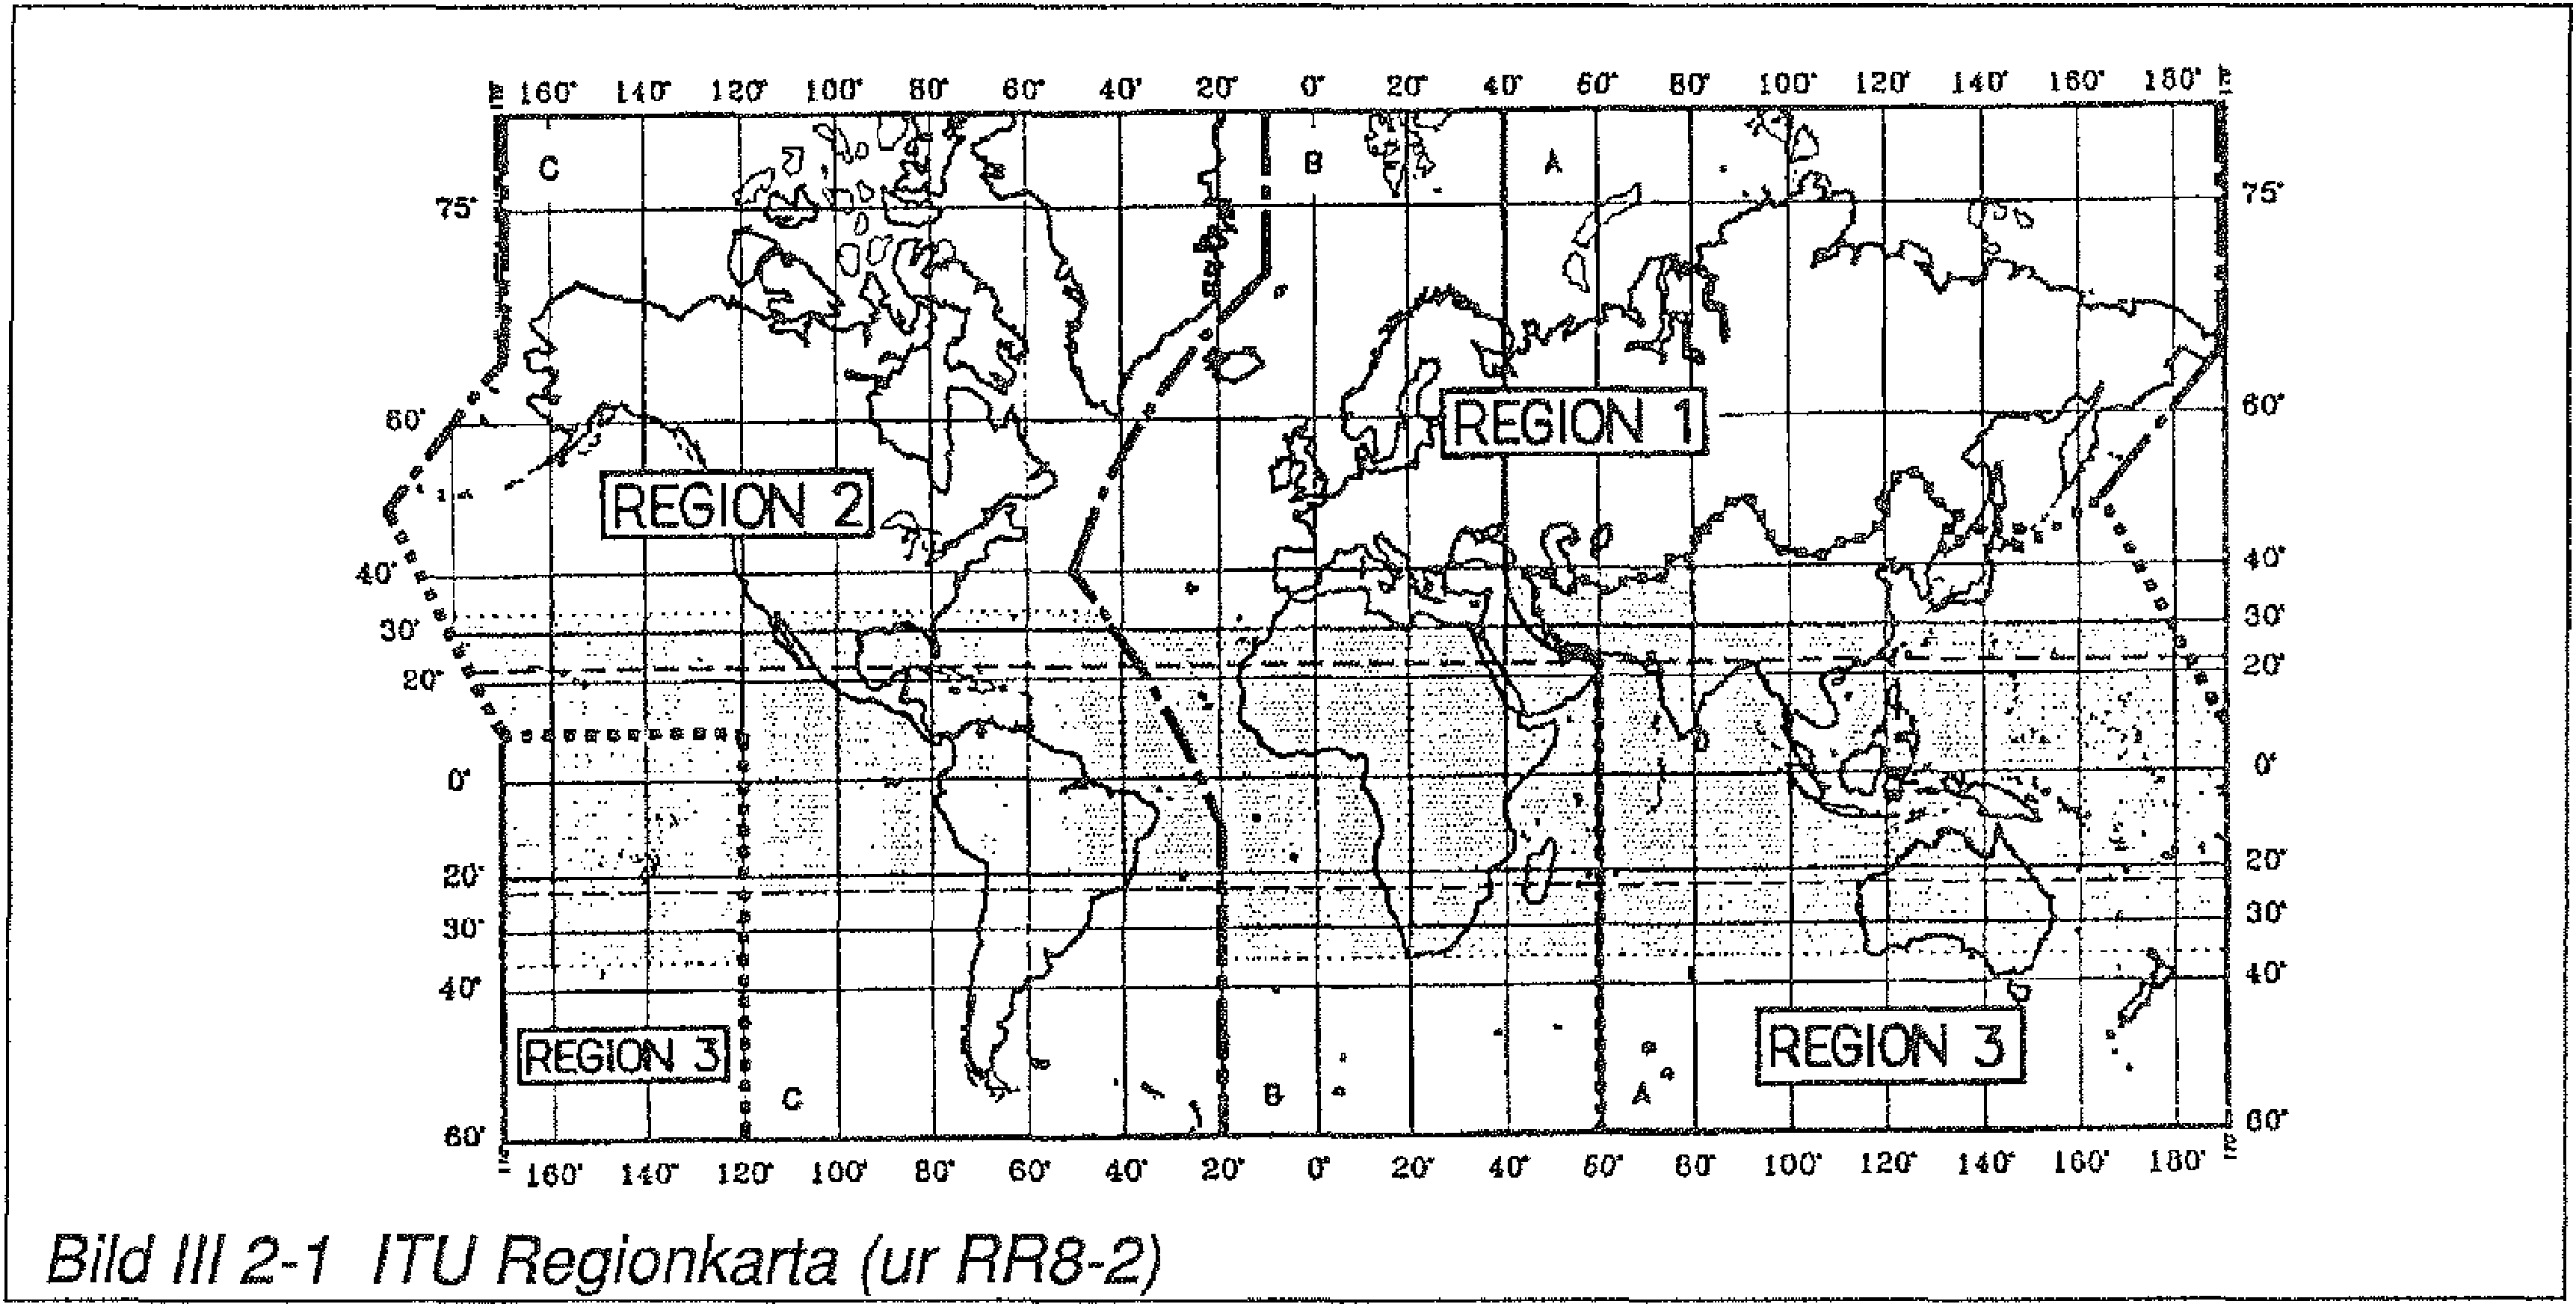
\includegraphics[width=\textwidth]{images/bild_3_2-01}
  \caption{ITU Regionkarta (ur RRB-2)}
  \label{fig:bildIII2-1}
\end{figure}
